\documentclass[10pt, a4paper]{report}

\usepackage[utf8]{inputenc}
\usepackage{polski}
\usepackage{a4wide}
\usepackage{fancyhdr}
\usepackage{lastpage}
\usepackage{tabularx}
\usepackage{listings}
\usepackage{graphicx}

\graphicspath{ {./images} }

%strona tytułowa
\begin{titlepage}

\title{\huge{\textbf{Sprawozdanie}}\\ gramatyk bezkontekstowych}
\author{Szymon Półtorak}
\date{}

\end{titlepage}

\renewcommand{\footrulewidth}{1pt}

\begin{document}
    \maketitle

    \renewcommand*\thesection{\arabic{section}} 
    
    \pagestyle{fancy}
    \fancyhf{}
    \rhead{Szymon Półtorak}
    \cfoot{Strona \thepage \hspace{1pt} z \pageref{LastPage}}
    
    \fancypagestyle{plain}{
        \rhead{Szymon Półtorak}
        \cfoot{Strona \thepage \hspace{1pt} z \pageref{LastPage}}
    }
    \tableofcontents
    \newpage

    \section{Treść Zadania}
    \begin{figure}[h]
        \begin{center}
            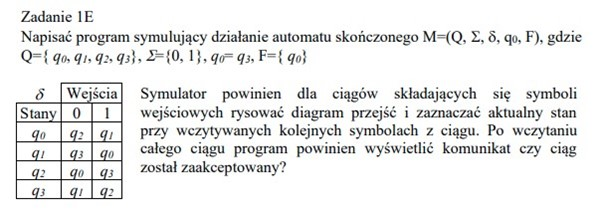
\includegraphics[scale=0.8]{photo1.jpg}
            \caption{mportowanie Projektu}
        \end{center}
    \end{figure}

    \section{Instrukcja Obsługi Programu}
    Program został napisany z myślą o współpracy z systemem Windows.
    Żeby uruchomić program trzeba wejść w program Visual Studio 2019 Enterprise i po załadowaniu projektu trzeba wybrać
    opcję „Local Windows Debugger”.

    \begin{figure}[h]
        \begin{center}
            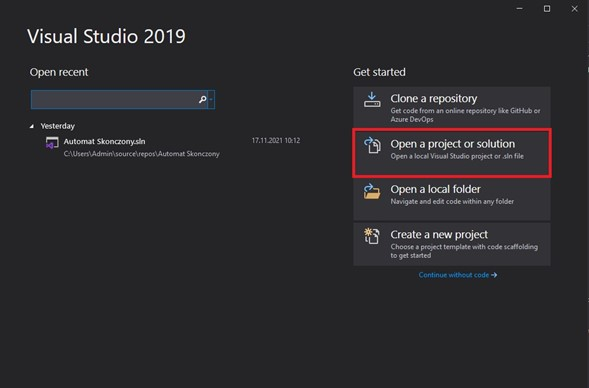
\includegraphics[scale=0.8]{photo2.jpg}
            \caption{mportowanie Projektu}
        \end{center}
    \end{figure}
    \newpage

    \begin{figure}[h]
        \begin{center}
            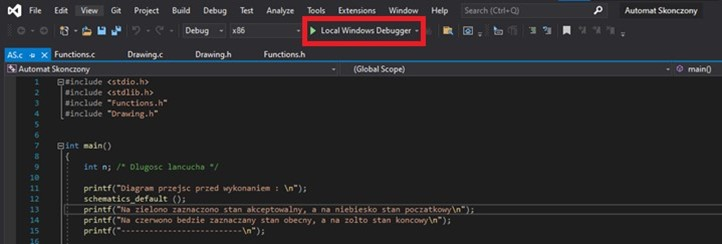
\includegraphics[scale=0.8]{photo3.jpg}
            \caption{mportowanie Projektu}
        \end{center}
    \end{figure}

    Po uruchomieniu programu w Visual Studio, ukaże się nam diagram przejść z zaznaczonym na zielono podwójnym kołem
    stanem końcowym oraz zaznaczonym na niebiesko i wskazywanym strzałką z napisem start stanem początkowym. Trzeba
    podać z klawiatury długość łańcucha jaki chcemy wprowadzić i zatwierdzić enterem. Następnie program poprosi nas o
    wprowadzenie łańcucha. Żeby to zrobić wpisujemy z klawiatury 0 lub 1 i zatwierdzamy wprowadzoną liczbę klawiszem enter.
    Jeżeli wprowadzimy liczbę różną od 0 i 1 program wyświetli komunikat o błędnym znaku i poprosi o wprowadzenie
    poprawnego. Czynność powtarzamy aż ich ilość będzie równa podanej przez użytkownika długości łańcucha. Po wpisaniu
    liczb program wyświetli wczytany łańcuch. Program zaczeka aż użytkownik kliknie jakikolwiek przycisk. Po jego wciśnięciu
    program wyświetli dokonane przejścia, a po kolejnych wciśnięciach klawisza będzie wyświetlał diagram przejść z
    zaznaczonymi kolejnymi przejściami automatu ( na czerwono ). Czynność powtarzamy aż pojawi się diagram z zaznaczonym
    na żółto stanem końcowym. Po następnym użyciu klawisza pojawi się informacja czy łańcuch został zaakceptowany. Program
    zakończy działanie po następnym użyciu dowolnego klawisza.

    \begin{figure}[h]
        \begin{center}
            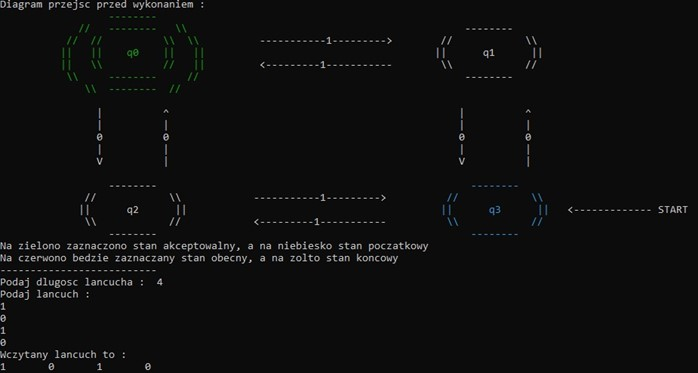
\includegraphics[scale=0.8]{photo4.jpg}
            \caption{mportowanie Projektu}
        \end{center}
    \end{figure}
    \newpage

    \section{Dwa zestawy taśm wejściowych i przykład ich wykorzystania}

    \begin{enumerate}
        \item Przykładowy input do taśmy wejściowej akceptującej wejście:
        \newline Długość łańcucha: 4
        \newline Łańcuch: 1 0 1 1

        \begin{figure}[h]
            \begin{center}
                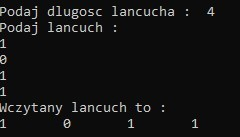
\includegraphics[scale=1]{photo5.jpg}
                \caption{mportowanie Projektu}
            \end{center}
        \end{figure}
        
        \item Przykładowy input do taśmy wejściowej nie akceptującej wejście:
        \newline Długość łańcucha: 5
        \newline Łańcuch: 1 1 0 0 1

        \begin{figure}[h]
            \begin{center}
                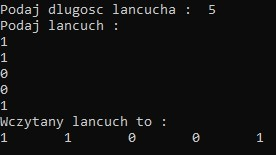
\includegraphics[scale=1]{photo6.jpg}
                \caption{mportowanie Projektu}
            \end{center}
        \end{figure}
        
    \end{enumerate}

    \section{Bibliografia}
    \begin{enumerate}
        \item \textit{Język ANSI C}, Brian W. Kernighan, Dennis M. Ritchie,
        \item \textit{Wprowadzenie do teorii automatów, języków i obliczeń}, John Hopcroft, Jeffrey Ullman.
    \end{enumerate}

\end{document}